\chapter{Analyse et conception}
\label{ch:analysis_design}

% =============================
% INTRODUCTION
% =============================
\section{Introduction}
L'objectif de ce chapitre est de traduire les besoins fonctionnels et non fonctionnels, identifiés lors de la phase d'analyse, en une solution technique détaillée et structurée. Cette étape de conception est cruciale car elle permet de définir l'ossature du système avant l'implémentation. Nous détaillerons ici les choix architecturaux, le formalisme de modélisation adopté ainsi que les diagrammes UML qui décrivent tant la structure statique que le comportement dynamique de Certif-fun. Ces choix sont justifiés par la nécessité de répondre aux exigences de scalabilité, de performance en temps réel et de sécurité propres à une plateforme de certification intelligente.

\section{Formalisme de modélisation : UML}
\subsection{Motivation et choix}
UML (\textit{Unified Modeling Language}) est un langage visuel standardisé pour modéliser un système logiciel. Il offre un ensemble de diagrammes (classes, cas d’utilisation, séquence, etc.) permettant de représenter précisément l’architecture, le comportement et les interactions complexes du système \cite{deshmukh2023uml}.

\begin{figure}[H]
    \centering
    
\includegraphics[width=0.2\linewidth]{figures/UML_logo.png}
    \caption{Logo du formalisme UML utilisé pour la modélisation.}
    \label{fig:uml_logo}
\end{figure}

L'utilisation de ce formalisme pour Certif-fun répond à plusieurs objectifs :
\begin{itemize}
    \item Description de la structure et du comportement : UML permet de visualiser le système sous plusieurs angles (statique avec les classes, dynamique avec les séquences).
    \item Communication efficace : Il sert de langage commun entre les intervenants du projet pour lever toute ambiguïté sur les flux de données.
    \item Garantie de cohérence et maintenabilité : Une conception rigoureuse facilite l'évolution future du code et identifie les incohérences logiques.
\end{itemize}

\subsection{Diagrammes retenus}
Dans le cadre de ce projet, nous avons retenu les diagrammes suivants pour formaliser notre conception :
\begin{itemize}
    \item Diagramme de classes : Pour représenter la structure statique des entités (Utilisateurs, Cours, Certificats) et leurs relations.
    \item Diagrammes de séquence : Pour illustrer les interactions complexes entre les microservices (ex: processus de surveillance Proctoring).
    \item Diagramme de déploiement : Pour visualiser l'organisation physique des composants (conteneurs Docker, bases de données) sur l'infrastructure.
\end{itemize}

% =============================
% ARCHITECTURE LOGICIELLE
% =============================
\section{Architecture logicielle}
Cette section décrit l’architecture globale du système, en distinguant clairement l’approche adoptée et en expliquant la répartition fonctionnelle et technique du code.

\subsection{Approche architecturale}
Pour le projet Certif-fun, nous avons confronté deux approches majeures : l'architecture monolithique et l'architecture microservices.

\begin{itemize}
    \item \textbf{Architecture monolithique :} Il s'agit d'une architecture traditionnelle où toutes les fonctionnalités d’une application sont réunies dans un seul programme. Tous les composants sont interdépendants et exécutés dans un même processus \cite{elgheriani2022differential}. Bien qu'elle offre une simplicité initiale, elle présente des inconvénients majeurs en termes de maintenance et de scalabilité ; dans notre cas, la charge de l'IA ralentirait l'ensemble de la plateforme.
    
    \item \textbf{Architecture microservices :} C'est une architecture qui divise une application en petits services autonomes pouvant être développés, déployés et mis à l’échelle indépendamment. Chaque service remplit une fonction métier spécifique et communique via des API bien définies \cite{bozic2023microservices}. Ce choix s'est imposé comme une évidence pour Certif-fun, offrant une scalabilité fine (pour le service IA), une isolation des pannes et une flexibilité technologique (Java/Spring Boot pour le métier et Python/FastAPI pour l'IA).
\end{itemize}

\subsection{Schéma de l'architecture et organisation en couches}
L'architecture de Certif-fun est conçue selon un modèle multicouche qui favorise la séparation des préoccupations et la modularité. Le schéma suivant illustre l'organisation globale du système :

\begin{figure}[H]
    \centering
    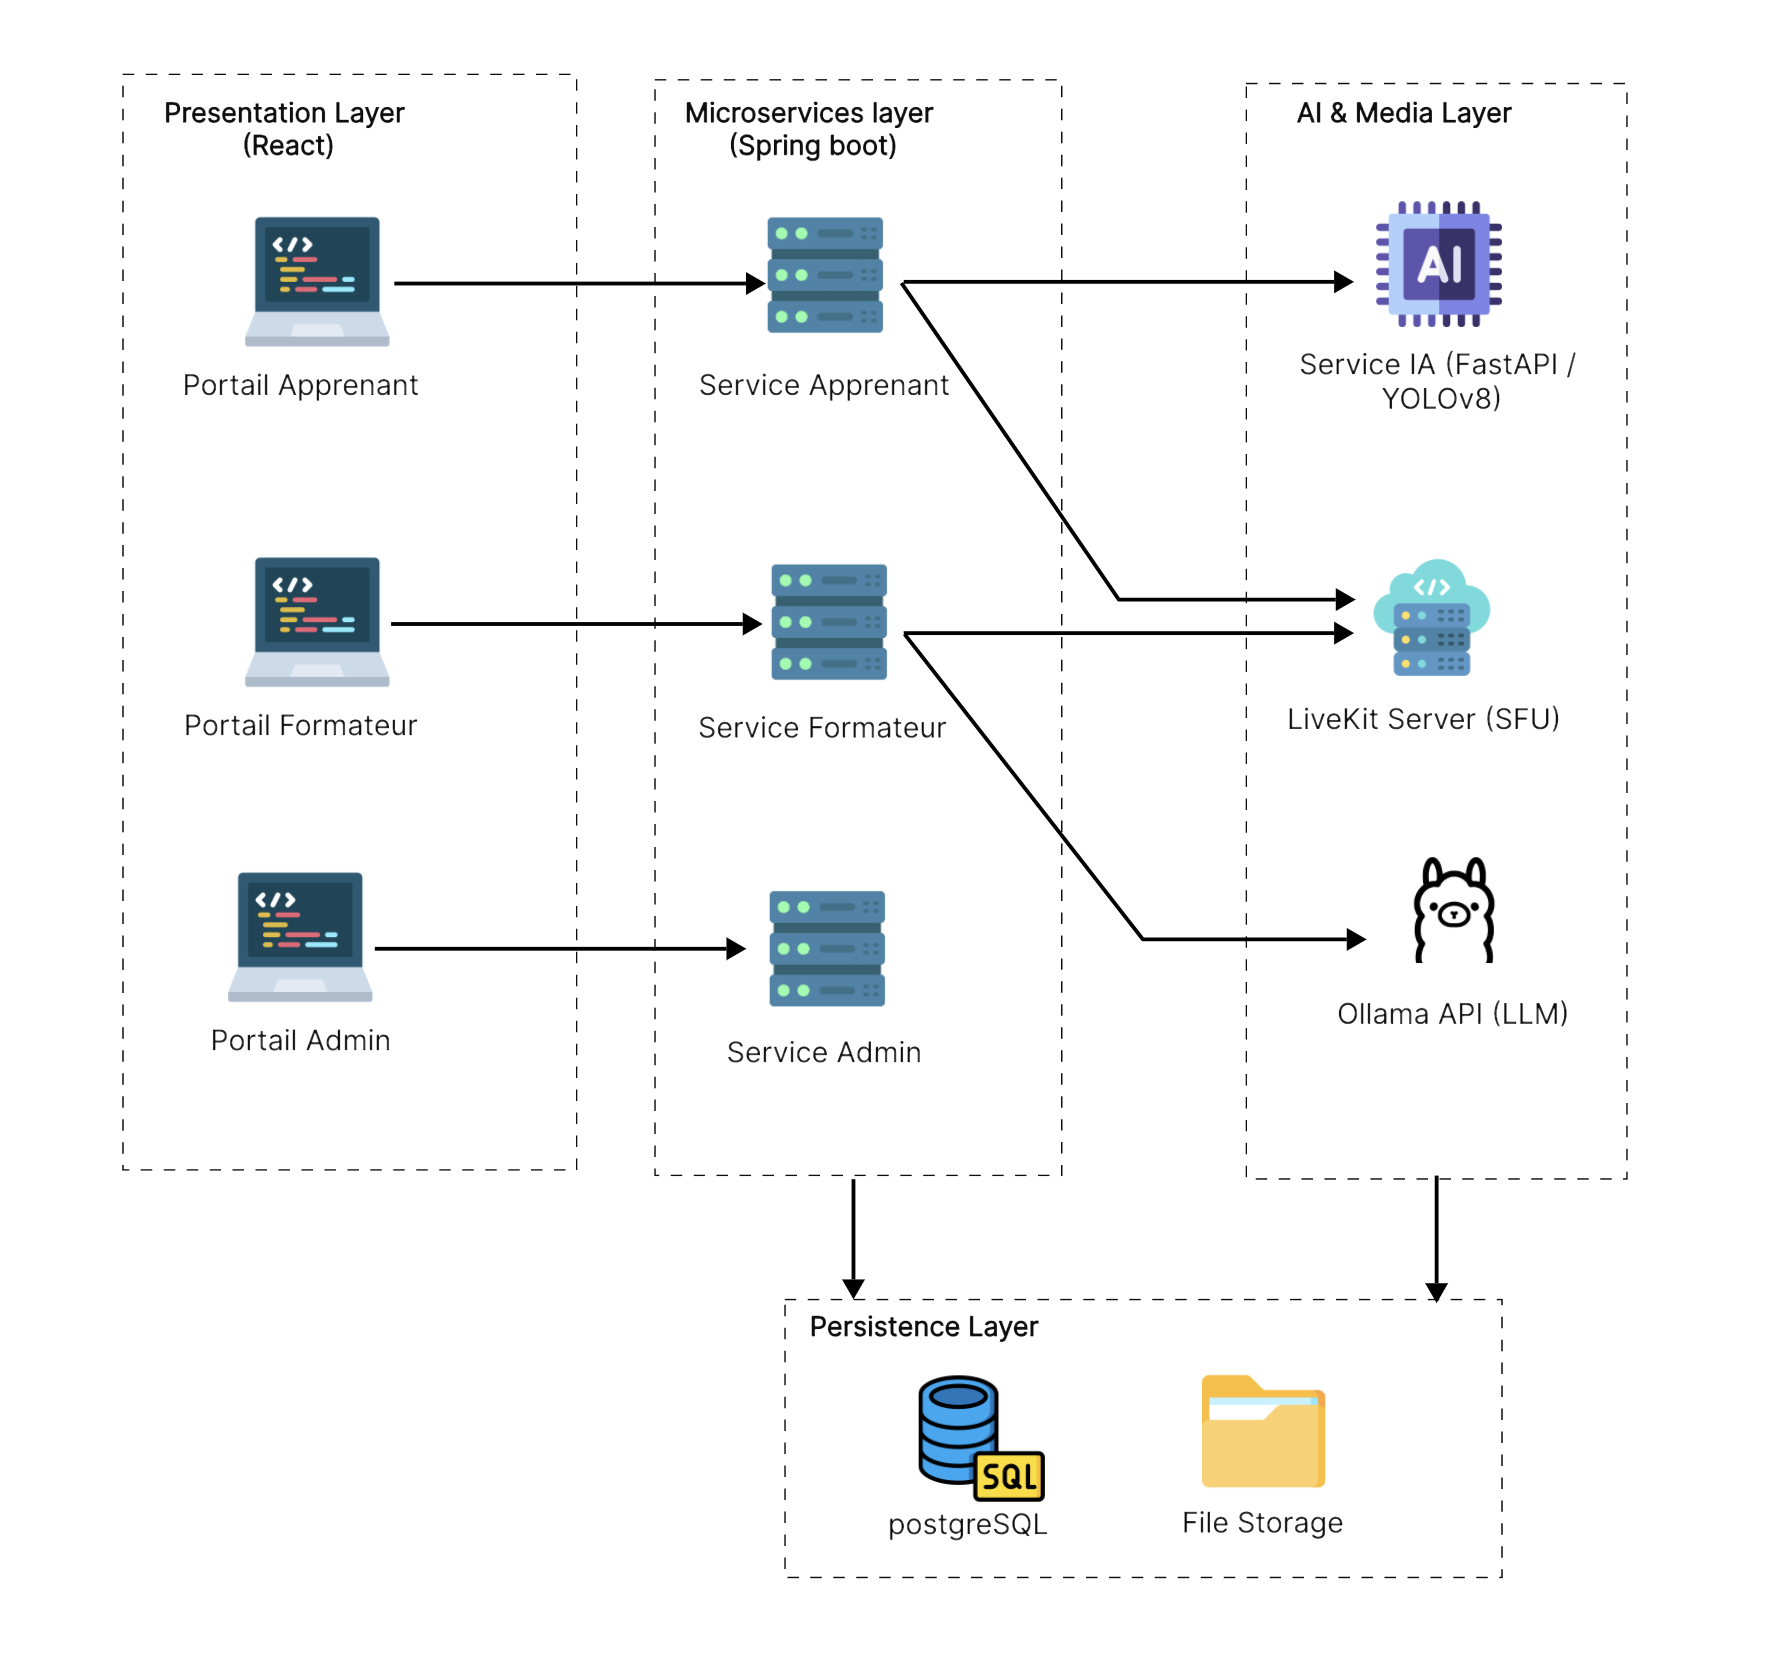
\includegraphics[width=1\linewidth]{figures/architecture_globale.png}
    \caption{Schéma de l'architecture globale du système Certif-fun.}
    \label{fig:architecture_globale}
\end{figure}

Comme illustré dans le diagramme ci-dessus, le système s'articule autour de quatre couches majeures :
\begin{itemize}
    \item Presentation Layer (React) : Regroupe les trois portails web (Apprenant, Formateur, Admin) qui servent d'interface utilisateur unique pour chaque profil.
    \item Microservices Layer (Spring Boot) : Constitue le cœur métier du système. Chaque service gère un domaine spécifique (Utilisateurs, Cours, Encadrement) et communique de manière isolée.
    \item AI \& Media Layer : Cette couche spécialisée gère les traitements lourds. Elle inclut le service de surveillance IA (FastAPI/YOLOv8), la visioconférence (LiveKit SFU) et la génération de contenu (Ollama LLM).
    \item Persistence Layer : Assure la conservation des données via PostgreSQL et le stockage des fichiers numériques (vidéos, ressources).
\end{itemize}

\subsection{Discussion}
Cette architecture répond aux besoins stratégiques du projet :
\begin{itemize}
    \item Maintenabilité : Le découpage permet de modifier un service (ex: mettre à jour le modèle IA) sans impacter les portails d'administration.
    \item Scalabilité : Face à une session d'examen massive, nous pouvons multiplier les instances du microservice de surveillance sans surcharger les autres services.
    \item Sécurité : L'utilisation de tokens JWT entre les couches garantit que les communications sont sécurisées et que les droits d'accès sont strictement respectés.
\end{itemize}

% =============================
% DIAGRAMMES DE CONCEPTION
% =============================
\section{Diagrammes de conception}
Cette section détaille les différents diagrammes qui ont servi à formaliser la conception du système.

\subsection{Diagramme de classes}
Le diagramme de classes est un diagramme UML structurel qui représente l'architecture statique d'un système orienté objet. Il est couramment utilisé pour modéliser les concepts, les données et les entités logiques du système \cite{miro_class_diagram}. Le diagramme suivant présente cette structure pour le système Certif-fun, détaillant les entités, leurs attributs ainsi que les relations qui les unissent.

\begin{figure}[H]
    \centering
    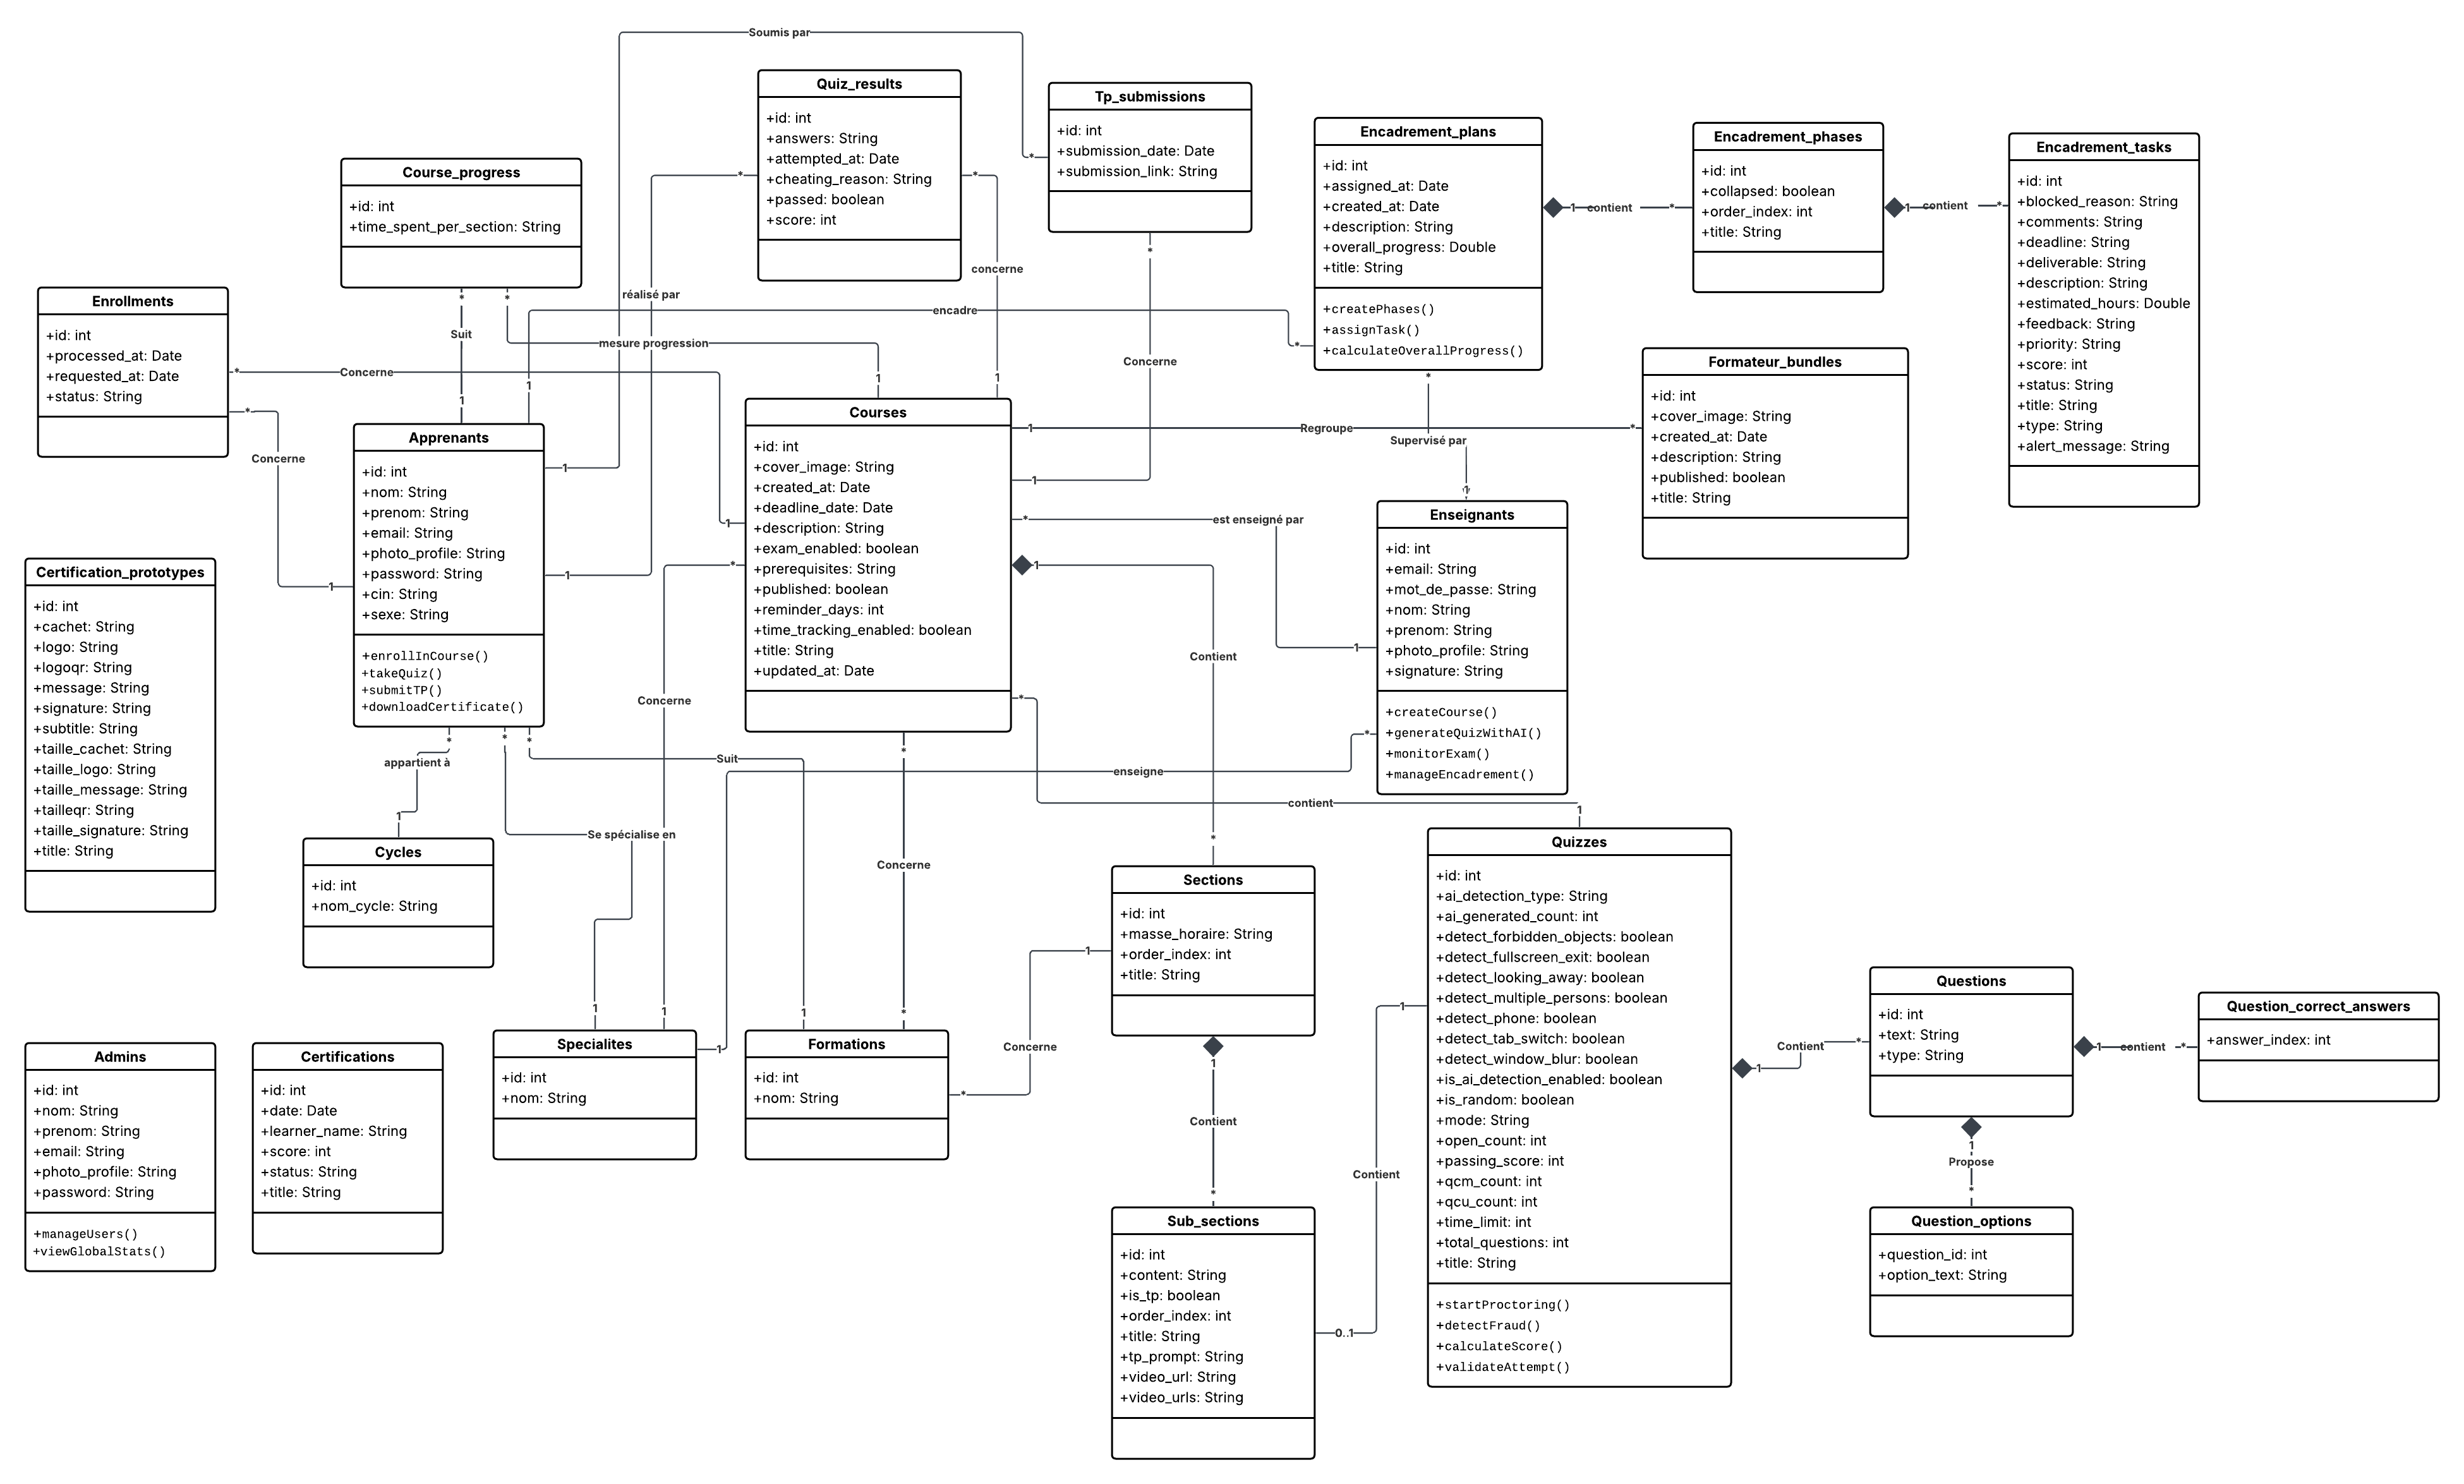
\includegraphics[width=1\linewidth]{figures/diagramme_classes.png}
    \caption{Diagramme de classes global de la base de données certif\_db.}
    \label{fig:diagramme_classes}
\end{figure}

\subsection{Analyse détaillée des entités et de leurs rôles métier}
Cette section détaille les responsabilités de chaque entité au sein de l'écosystème Certif-fun.

\paragraph{A. Gestion des Acteurs et de la Sécurité}
\begin{itemize}
    \item Classe Apprenant : C'est l'acteur central du système. Son rôle est de consommer le contenu pédagogique et de réaliser les examens finaux.
    \item Classe Enseignant (Formateur) : Il agit en tant qu'architecte pédagogique et mentor, concevant les parcours et assurant le suivi.
\end{itemize}

\paragraph{B. Structure Pédagogique et Contenu}
\begin{itemize}
    \item Classe Course (Cours) : Unité d'enseignement pivot entre les formateurs et les apprenants.
    \item Classe Section \& SubSection : Permettent un découpage logique et progressif du savoir (vidéo, texte, quiz).
    \item Classe FormateurBundle : Permet de créer des parcours thématiques regroupant plusieurs cours.
\end{itemize}

\paragraph{C. Évaluation Intelligente (IA \& Proctoring)}
\begin{itemize}
    \item Classe Quiz : Définit le cadre de l'examen final et porte les règles de surveillance IA (fraude, temps limite).
    \item Classe QuizResult : Conserve la trace de la performance et des alertes générées par l'IA.
\end{itemize}

\paragraph{D. Module d'Encadrement de Projet}
\begin{itemize}
    \item Classe EncadrementPlan : Structure la relation de tutorat et définit les objectifs du projet.
    \item Classe EncadrementTask : Représente une action concrète à réaliser (livrables et feedbacks).
\end{itemize}

\paragraph{E. Certification et Persistance}
\begin{itemize}
    \item Classe Certification : Aboutissement du processus attestant officiellement de la réussite.
    \item Classe CertificationPrototype : Gère l'aspect visuel, la mise en page et le format de signature.
\end{itemize}

\subsection{Diagrammes de séquence}
Le diagramme de séquence est un diagramme UML comportemental d'interaction qui montre comment les différents objets ou acteurs d'un système coopèrent en échangeant des messages au fil du temps \cite{miro_sequence_diagram}. Les diagrammes suivants illustrent cette dynamique pour Certif-fun.

\subsubsection{Passage d'examen avec surveillance IA (Proctoring)}
Ce diagramme détaille le flux de surveillance en temps réel. Pendant que l'apprenant répond aux questions, son flux vidéo est analysé par YOLOv8 pour détecter toute fraude (téléphone, absence) et alerter immédiatement le backend.

\begin{figure}[H]
    \centering
    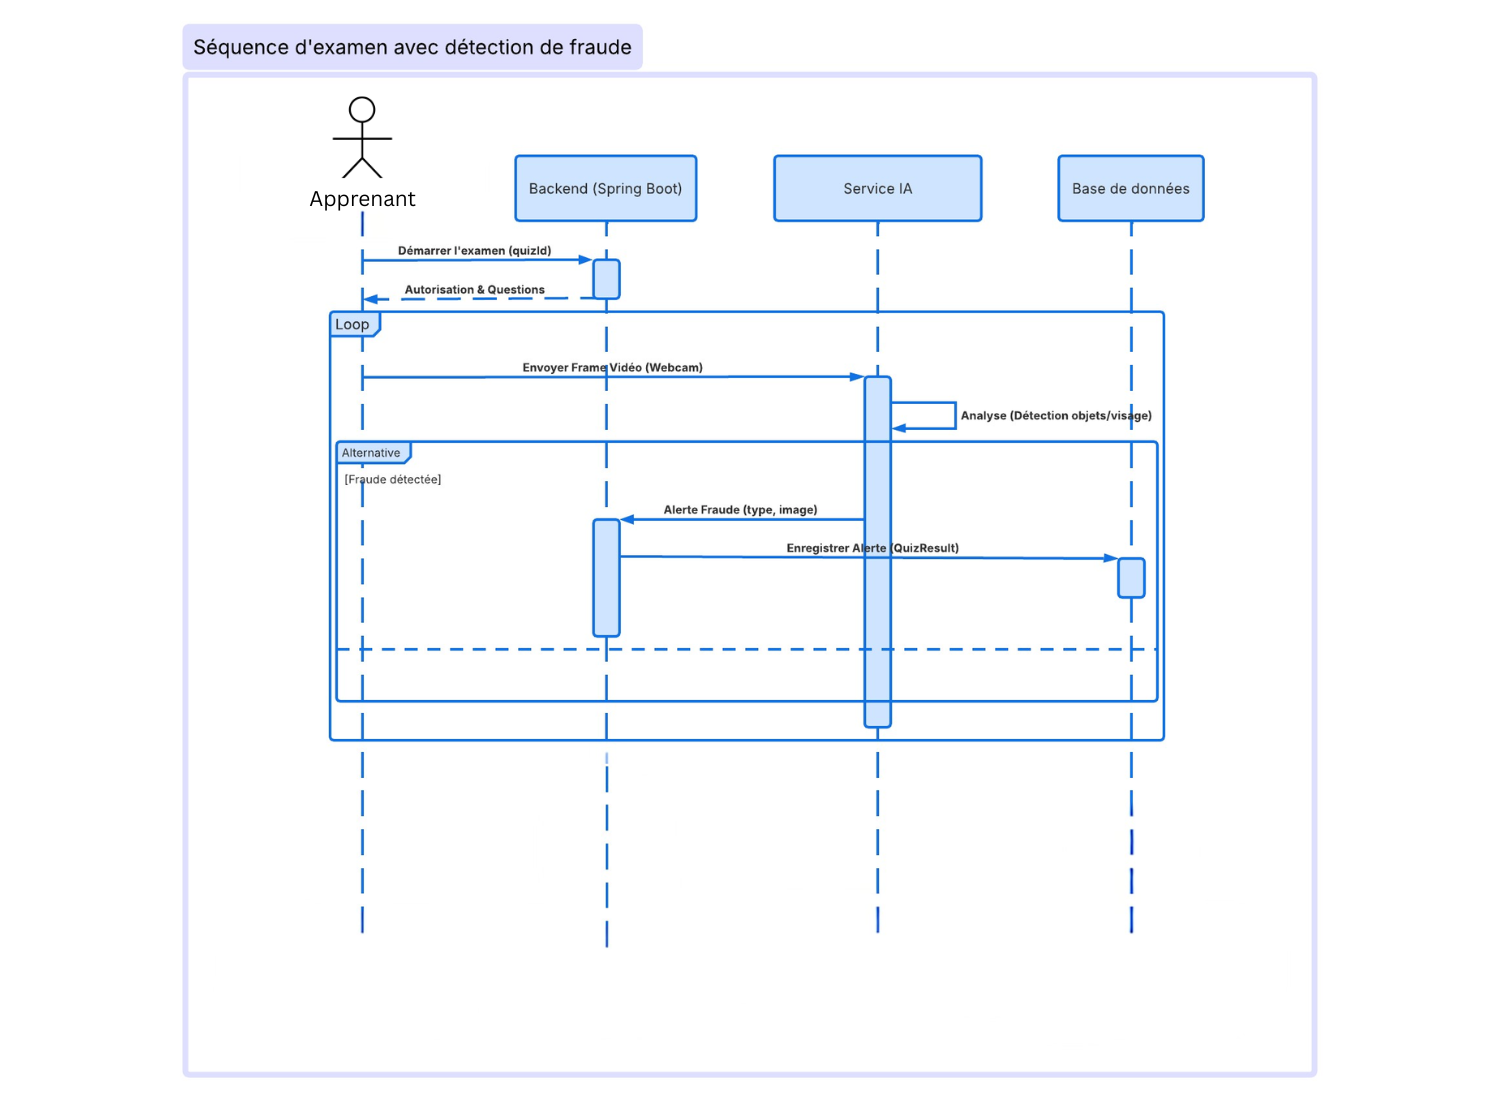
\includegraphics[width=0.9\linewidth]{figures/sequence1.png}
    \caption{Diagramme de séquence du processus de surveillance IA.}
    \label{fig:seq_proctoring}
\end{figure}

\subsubsection{Processus d'Encadrement et d'Évaluation}
Ce scénario illustre le cycle allant de la création d'une tâche d'encadrement à la soumission du livrable et au feedback du formateur, assurant un suivi pédagogique rigoureux.

\begin{figure}[H]
    \centering
    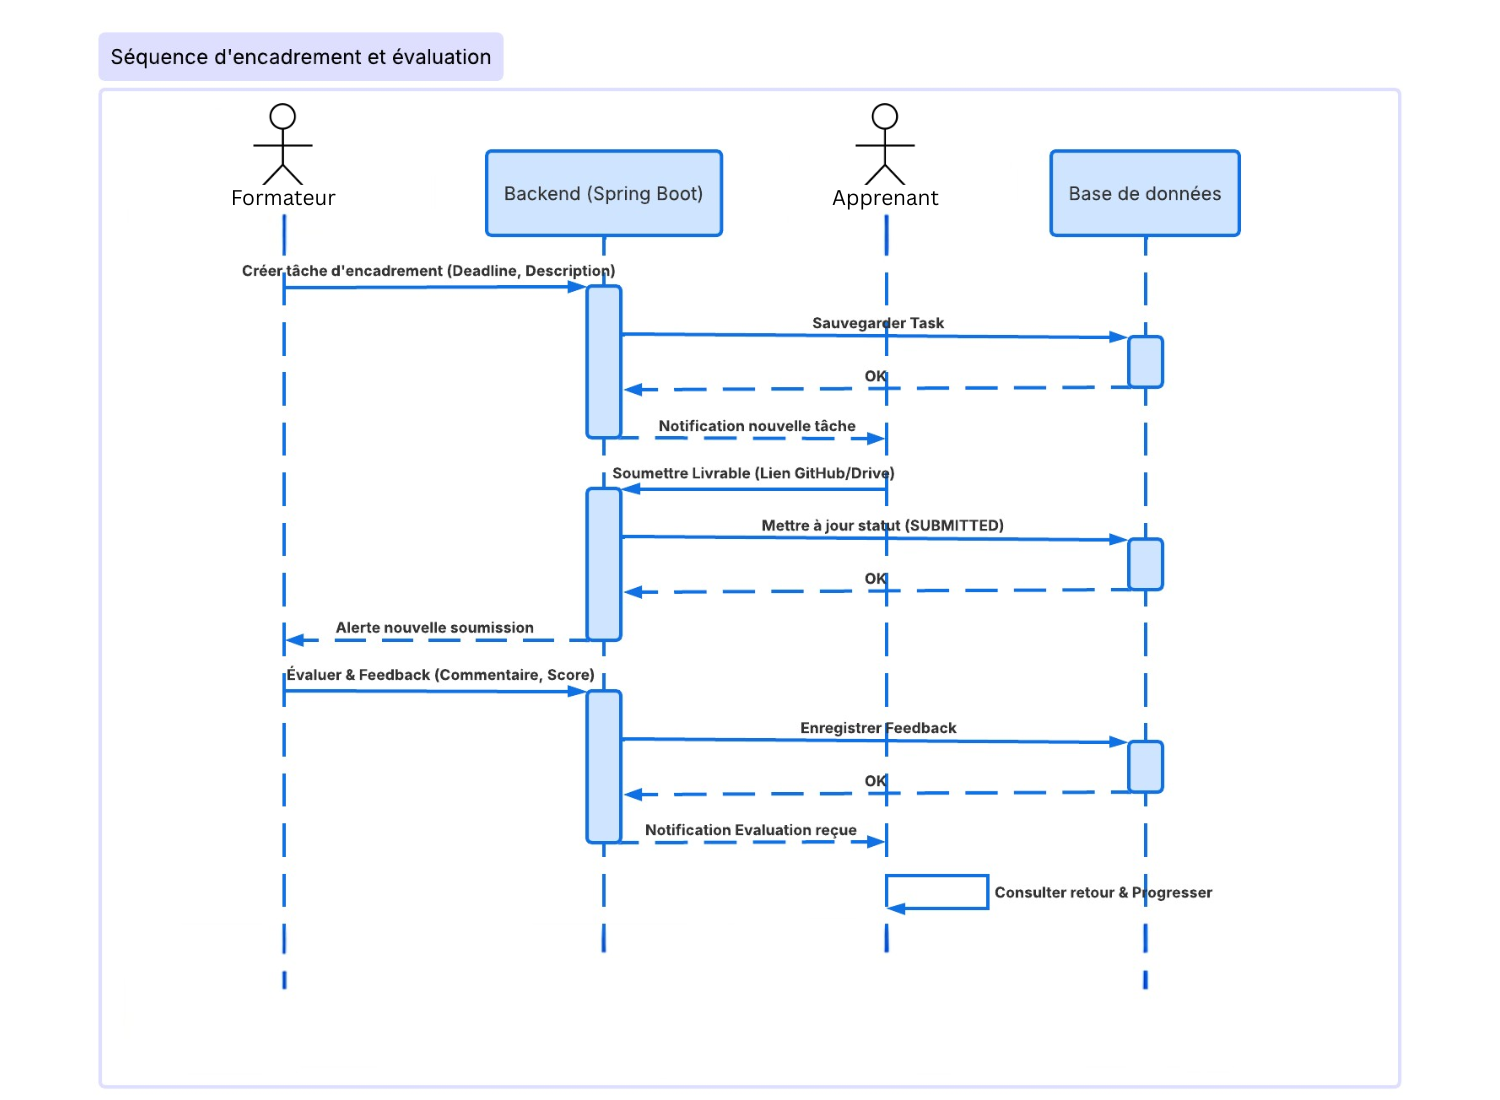
\includegraphics[width=0.9\linewidth]{figures/sequence2.png}
    \caption{Diagramme de séquence de l'encadrement et de l'évaluation.}
    \label{fig:seq_encadrement}
\end{figure}

\subsubsection{Génération de Quiz assistée par LLM (Ollama)}
Ce diagramme montre comment le backend prépare un prompt structuré pour Ollama afin de générer un quiz JSON prêt à être publié par l'enseignant.

\begin{figure}[H]
    \centering
    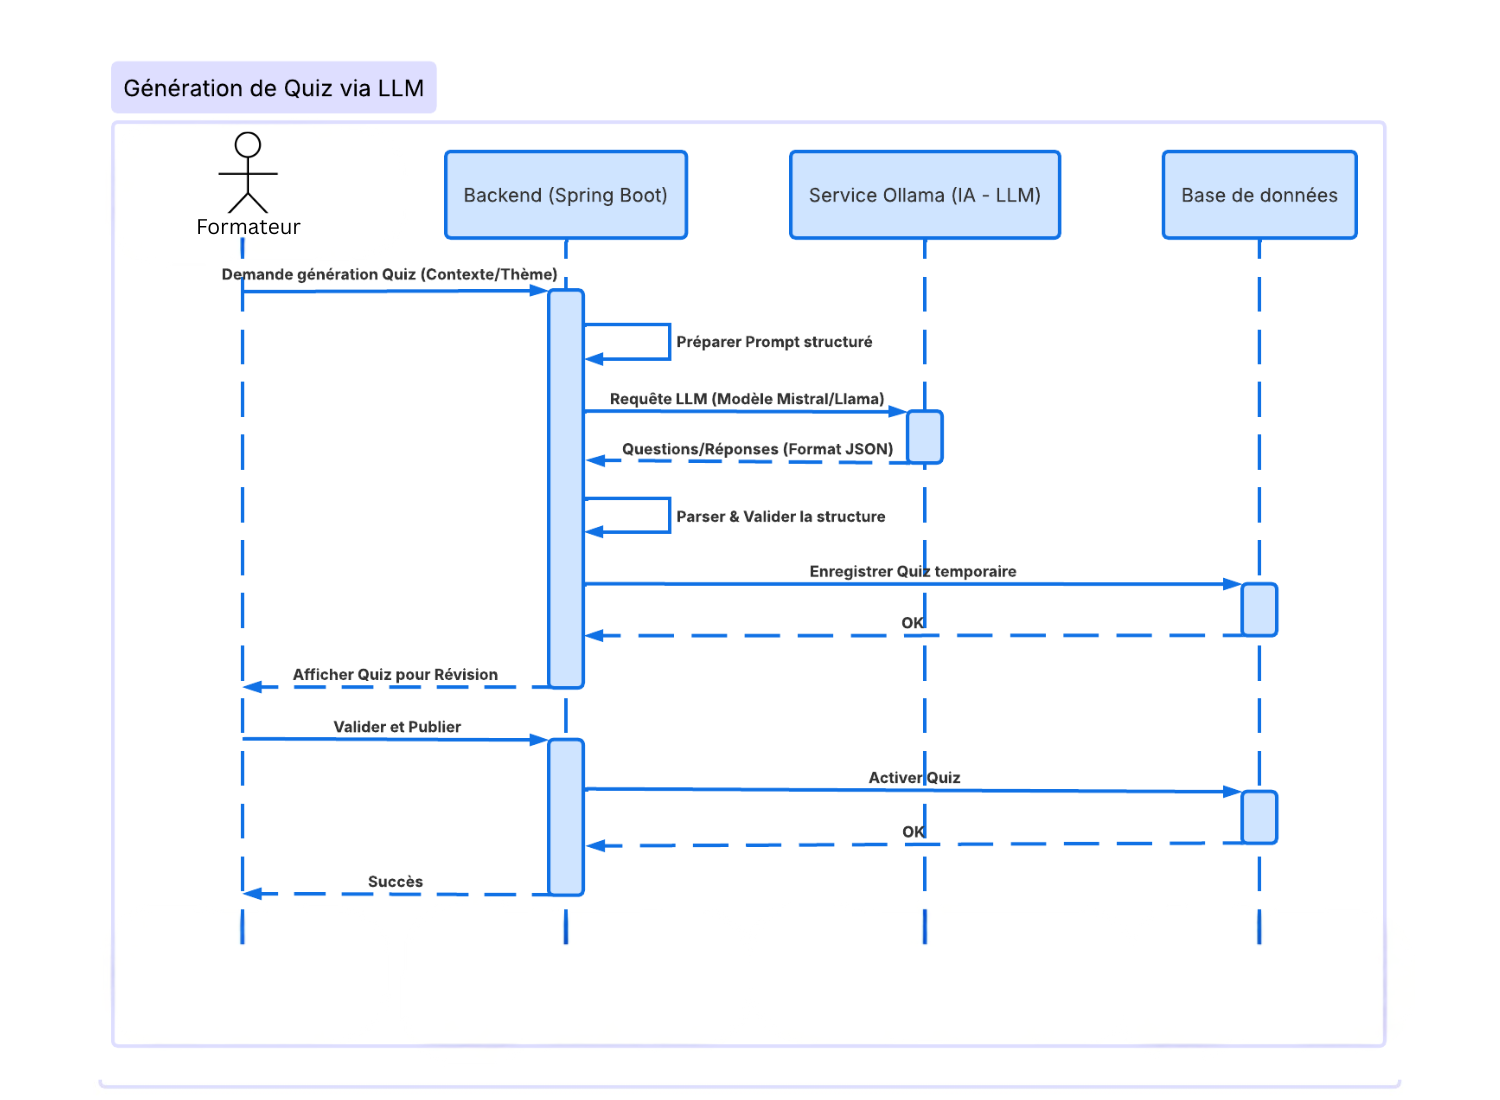
\includegraphics[width=0.9\linewidth]{figures/sequence3.png}
    \caption{Diagramme de séquence de la génération de quiz par LLM.}
    \label{fig:seq_ollama}
\end{figure}

\subsubsection{Visioconférence et Collaboration via LiveKit}
Ce scénario décrit la négociation WebRTC facilitée par le serveur LiveKit (SFU), assurant une distribution fluide et scalable des flux médias entre participants.

\begin{figure}[H]
    \centering
    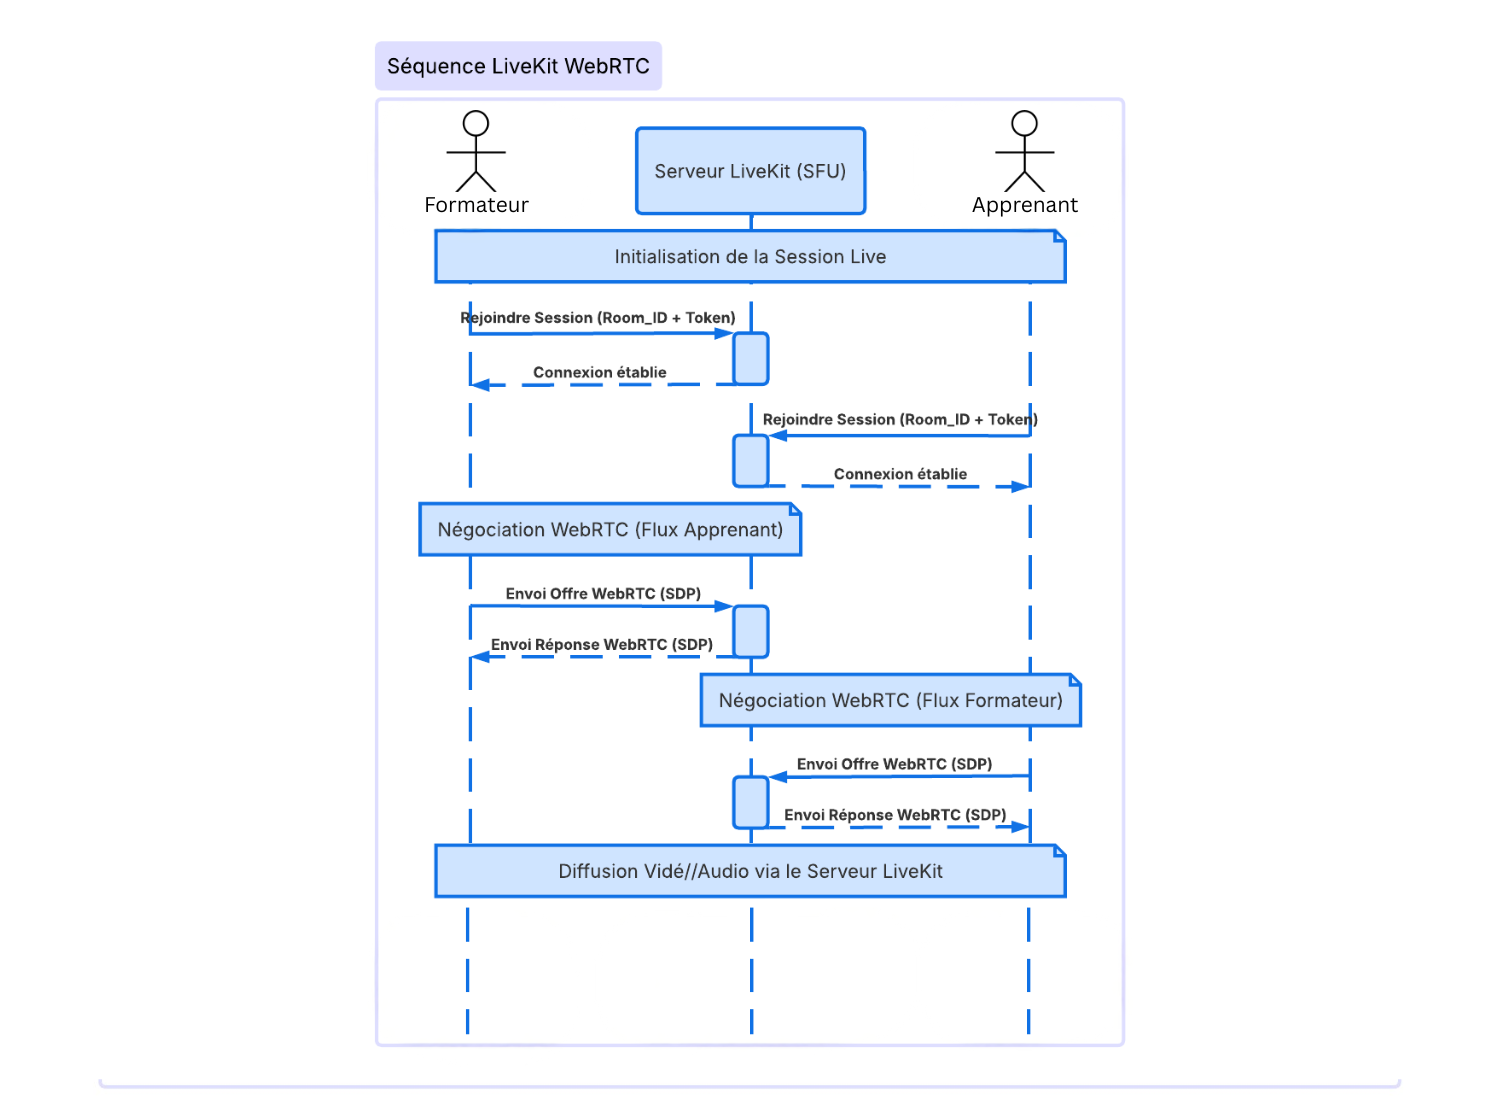
\includegraphics[width=0.85\linewidth]{figures/sequence4.png}
    \caption{Diagramme de séquence de la visioconférence WebRTC.}
    \label{fig:seq_livekit}
\end{figure}

\subsubsection{Authentification et Accès à l'Examen}
Ce diagramme détaille les quatre phases critiques du module de vérification d'identité : le scan du code QR pour la validation de l'inscription, la vérification de l'authenticité du document (carte d'étudiant), la reconnaissance faciale biométrique et enfin l'autorisation d'accès à l'examen.

\begin{figure}[H]
    \centering
    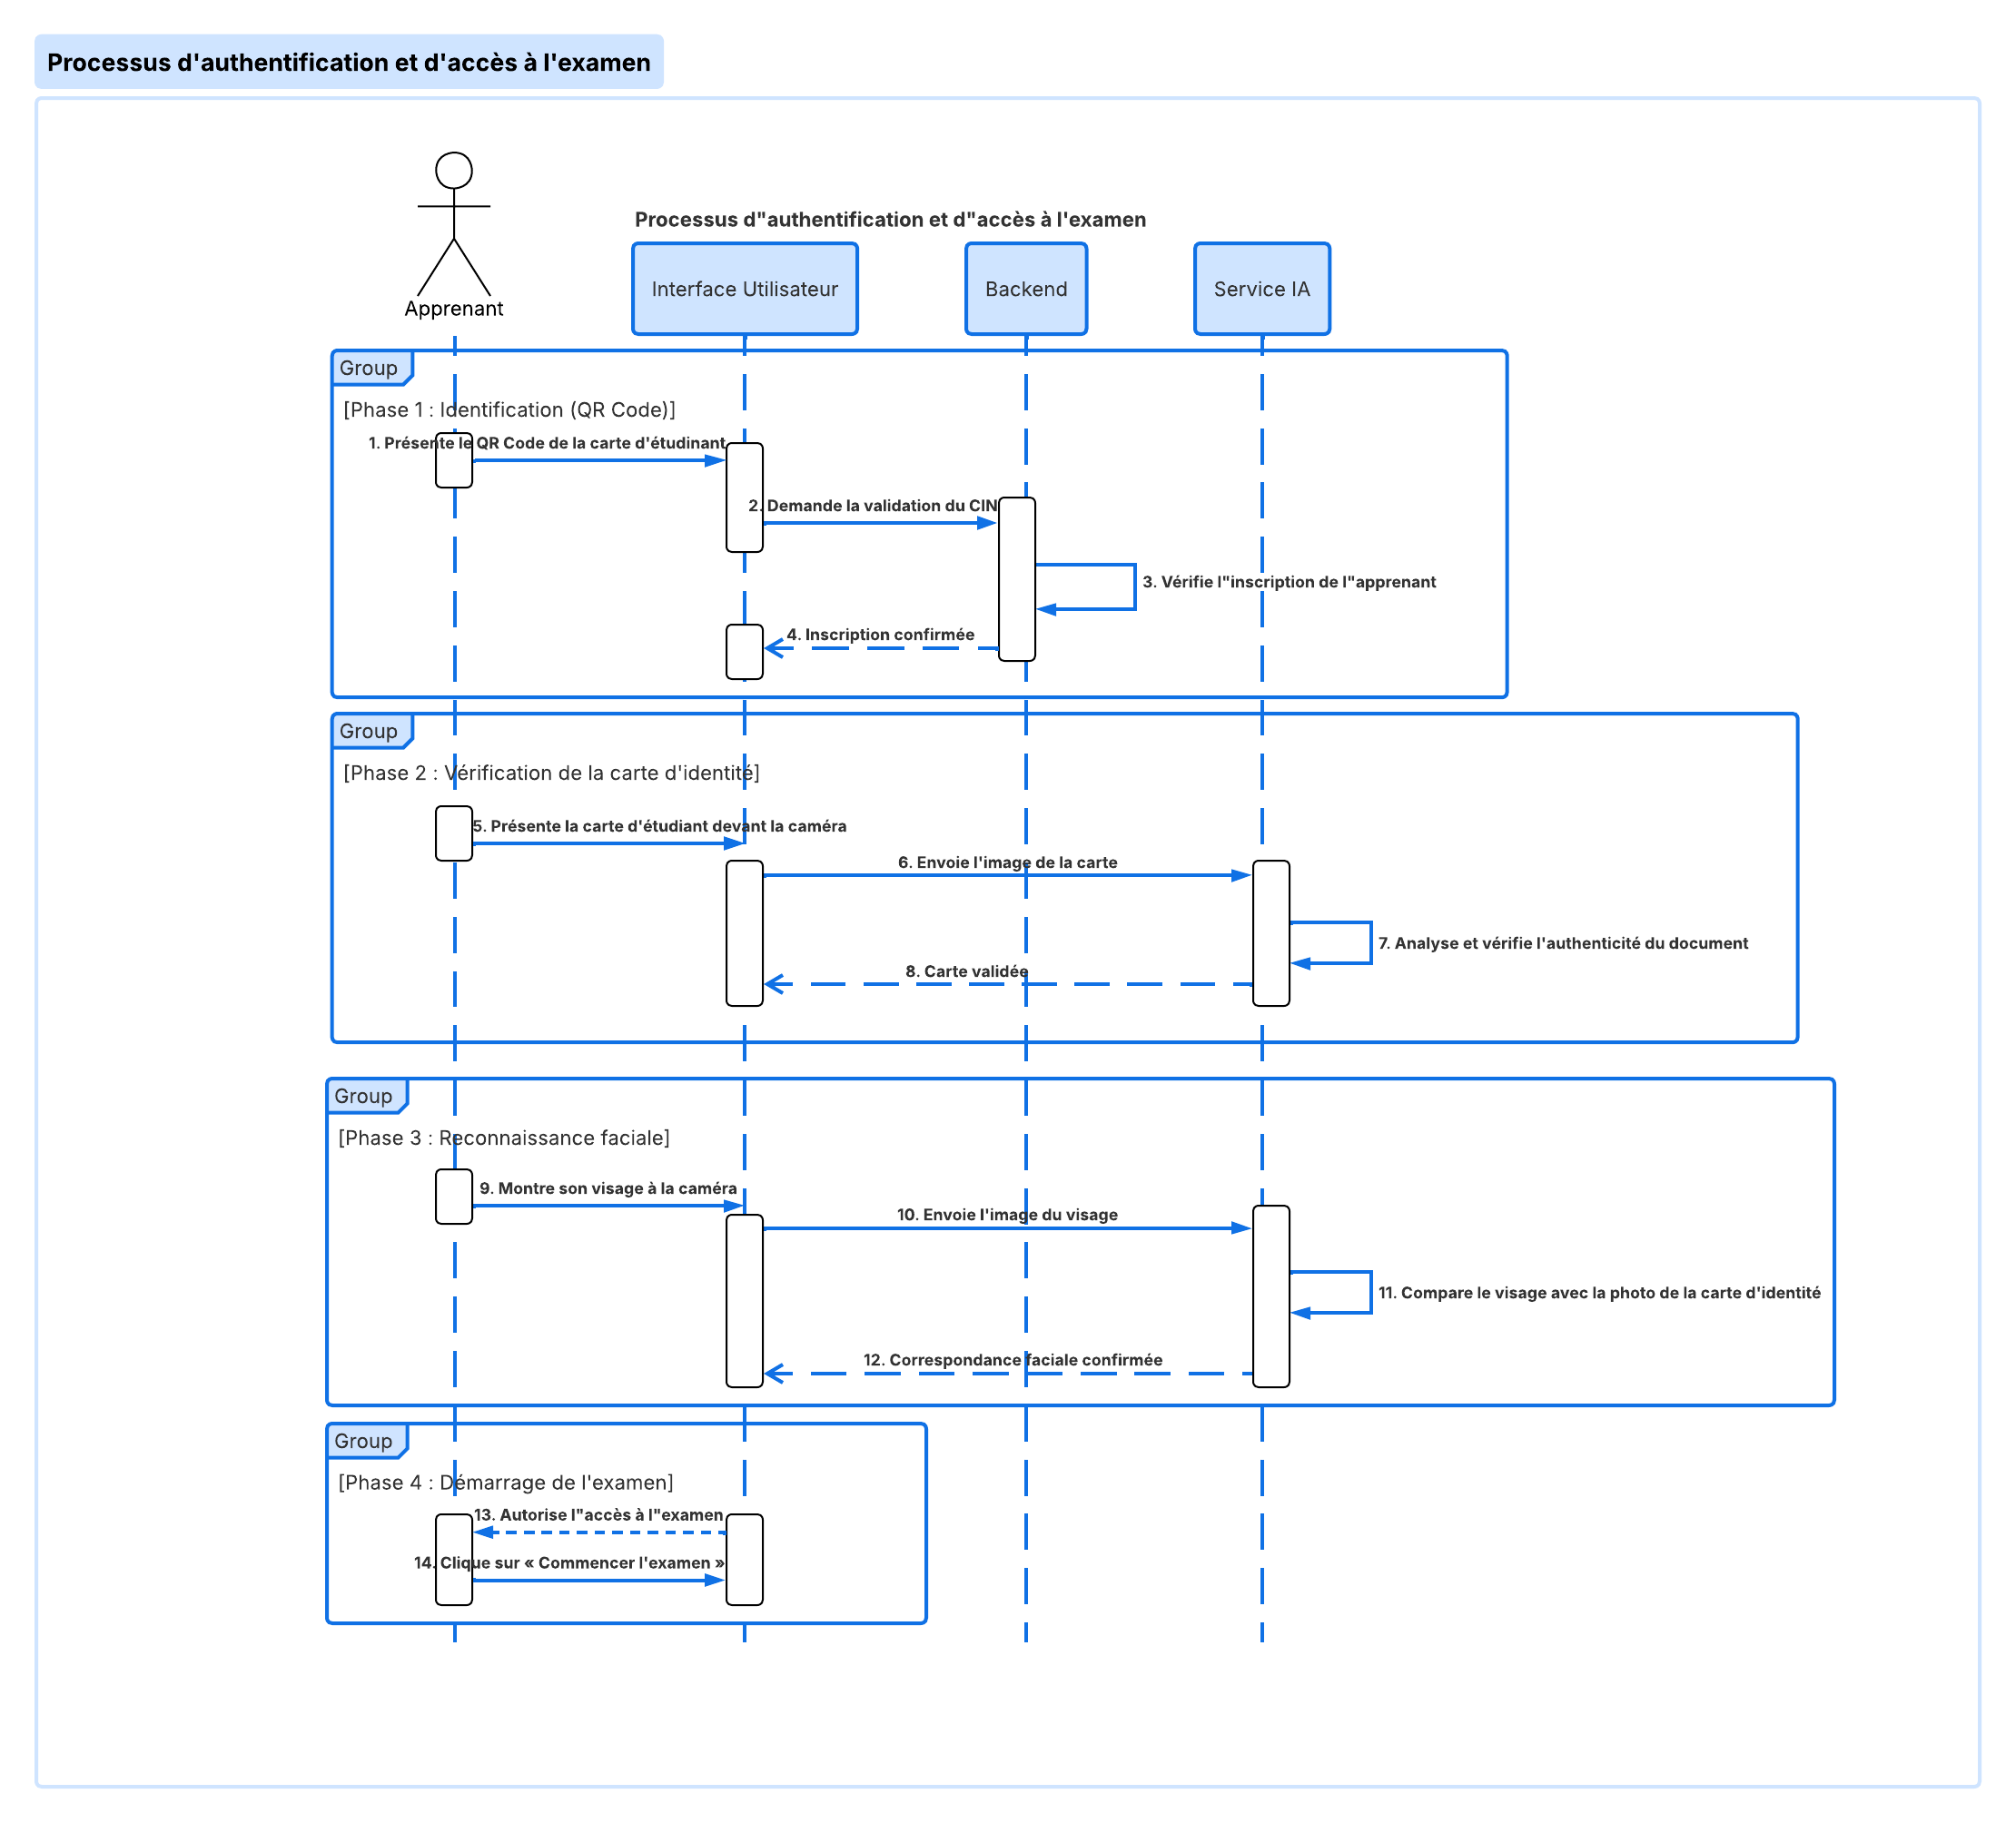
\includegraphics[width=0.98\linewidth]{figures/sequence5.png}
    \caption{Diagramme de séquence du processus d'authentification et d'accès à l'examen.}
    \label{fig:seq_auth_examen}
\end{figure}

\section{Conclusion}
En conclusion, ce chapitre a permis de poser les fondements techniques de la plateforme Certif-fun à travers une modélisation rigoureuse et une architecture microservices parfaitement adaptée aux enjeux du projet. Le choix du formalisme UML pour les diagrammes de classes et de séquences, combiné à une architecture découpée en couches fonctionnelles, garantit une séparation nette des responsabilités entre les modules. Cette structure facilite non seulement l'intégration de services complexes tels que la surveillance proactive par IA et la visioconférence en temps réel, mais elle simplifie également la maintenance et les évolutions futures du système. Ces décisions architecturales assurent une modularité optimale et répondent aux exigences critiques de performance, de haute disponibilité et de sécurité, indispensables à une plateforme de certification de ce calibre. Les modèles et schémas ainsi définis constituent le socle technique indispensable sur lequel s'appuiera la phase de réalisation pratique et de déploiement, dont les détails techniques et les interfaces seront présentés de manière approfondie dans le chapitre suivant.
